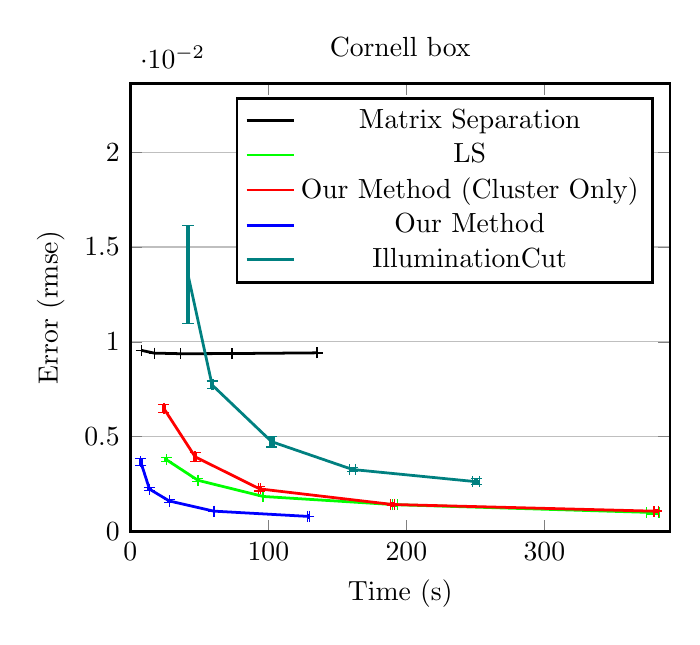
\begin{tikzpicture}
\begin{axis}[
title={Cornell box},
xlabel={Time (s)},
ylabel={Error (rmse)},
xmin=0, xmax=391.061,
ymin=0, ymax=0.02362764351320543,
legend pos=north east,
ymajorgrids=true,
error bars/y dir      = both,
error bars/y explicit = true,
error bars/x dir      = both,
error bars/x explicit = true,
error bars/error bar style={line width=1.5pt},
line width=1pt,
]

\addplot[
color=black,
]
coordinates {
(7.832237999999999, 0.009556036307563852) +- (0.07460450498461871, 5.938694516308629e-06)(17.32504, 0.009408484466333885) +- (0.05255201803927276, 3.901911233048198e-06)(36.1631, 0.00937784174928832) +- (0.13271942209036314, 2.136145949157021e-06)(73.55978, 0.009385488922265242) +- (0.1087857591783034, 7.759376812492812e-06)(135.44279999999998, 0.009423405987138204) +- (0.27917546453798514, 1.740873471746206e-05)
};
\addlegendentry{Matrix Separation}
\addplot[
color=green,
]
coordinates {
(26.08732, 0.0037926515549417533) +- (0.12568673517917495, 0.00010886853797962293)(48.95254, 0.00270607852322029) +- (0.3518523988833945, 7.505502478508069e-05)(96.35996, 0.0018533518009723846) +- (0.3945300934022661, 1.9893234612070887e-05)(191.8852, 0.0014208810171988957) +- (1.9221168382801266, 2.5219764007026227e-05)(378.43039999999996, 0.0010088391161440701) +- (4.649172051021552, 8.455747119201044e-06)
};
\addlegendentry{LS}
\addplot[
color=red,
]
coordinates {
(24.280520000000003, 0.006489197010975644) +- (0.30570383936090856, 0.00019363357405126087)(46.952760000000005, 0.003942383822102419) +- (0.41510398287658046, 0.00023267292568010173)(93.7153, 0.002252353003741484) +- (0.6911180362282557, 0.00011220306192173693)(189.948, 0.001431384666020364) +- (1.6909062954522336, 2.9520309896331312e-05)(381.05120000000005, 0.001076764543686928) +- (1.6246555450310076, 2.52418843238829e-05)
};
\addlegendentry{Our Method (Cluster Only)}
\addplot[
color=blue,
]
coordinates {
(7.512054000000001, 0.0036773453604919564) +- (0.08679751486073785, 0.00020003082266720294)(13.834340000000001, 0.002241616529037515) +- (0.16827090241631198, 7.402459521349906e-05)(28.188499999999998, 0.0016168932530926557) +- (0.0942153225330146, 7.08069690314297e-05)(60.33382, 0.0010818403560180646) +- (0.3341765931360241, 1.3898327333788267e-05)(129.1168, 0.0008019985926546482) +- (0.5374331958485632, 1.9498751078500818e-05)
};
\addlegendentry{Our Method}
\addplot[
color=teal,
]
coordinates {
(41.76264, 0.013539482760392763) +- (0.2332743547842323, 0.002574354425192581)(59.20532000000001, 0.007733129169919957) +- (0.6478153374226333, 0.00020847070541735242)(102.33337999999999, 0.004741671298992753) +- (1.7185541290282353, 0.0002827829758151285)(161.0142, 0.0032747160998119924) +- (2.0755298937861624, 0.00011970045946572997)(250.66979999999998, 0.002632092912411686) +- (2.5317079294420965, 0.00016094695578988788)
};
\addlegendentry{IlluminationCut}
\end{axis}
\end{tikzpicture}
